\chapter{Resultados y conclusiones.}


\hspace{0.4cm} Una vez obtenida la data para los Tif y Vebono se utiliz\'o la funci\'on ``smooth.spline" del programa estad\'istico R, para ajustar un spline c\'ubico a la data ingresada. Los argumentos requeridos por esta funci\'on son los siguientes,

\begin{itemize}
  \item X: representa el vector de la variable predictiva.
  \item Y: representa el vector de la variable repuesta.
  \item cv: (TRUE/FALSE) variable del tipo l\'ogico que representa si se va a utilizar la validaci\'on cruzada generalizada al momento de calcular el par\'ametro de suavizamiento.
  \item Spar: representa el par\'ametro de suavizamiento, t\'ipicamente (aunque no necesariamente) ubicado entre 0 y 1. Es el coeficiente lambda que acompa\~na a la integral del cuadrado de la segunda derivada de la funci\'on f.
\end{itemize}


\hspace{0.4cm} De esta manera el siguiente comando ajusta un spline cubico a la data ingresada,\\

spline1=smooth.spline(X=datT1\$Plazo,Y=datT1\$Rendimiento,cv=TRUE, spar=1.35)\\


\noindent y lo guarda en la variable ``spline1".\\

\hspace{0.4cm} Es importante se\~nalar lo crucial de la escogencia del par\'ametro ``spar", pues de \'el depende que tan suave sea la curva, la Figura 9 muestra como var\'ia la curva ajustada a la data de los Vebonos para la versi\'on 2 y con fecha de valoraci\'on $02-06-17$, cuando se var\'ia el ``spar", para esta comparaci\'on se us\'o tres valores, el primero fue 0.51 con el cual se obtiene una curva con ciertos picos la cual no es suave en lo absoluto. Usando el valor de 0.71 se obtiene la curva roja la cual presenta una mayor suavidad. Mientras que usando el valor de 0.81 se obtiene un mejor resultado aunque similar al anterior.


% \begin{figure}[h]
%   {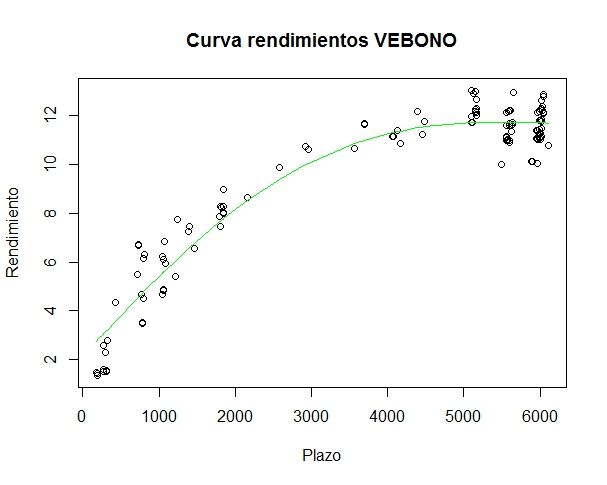
\includegraphics{images/curvarend.jpeg}}
% \caption{Curva de rendimiento Vebono versi\'on 2 para diferentes valores de suavizado.}
% \end{figure}


\hspace{0.4cm} Por su parte la Figura 10, muestra una comparaci\'on entre las curvas obtenidas al variar el ``spar" para el caso de la data de los Vebonos usando la versi\'on 3 y con fecha de valoraci\'on $10-08-17$. En la misma se aprecian 572 observaciones. Para el valor de 0.51 se obtiene la curva negra la cual presenta muchas oscilaciones, para el valor 0.90 (curva roja) se observa una mejor\'ia en la curva pero la misma no es suave. Finalmente para el valor de 1.20 se obtiene una curva suave (curva azul).


\hspace{0.4cm} Una vez que se obtiene la curva estimada y es guardada en una variable (en este caso, la variable es spline1), se procede a aplicar el comando ``predict", para estimar el rendimiento de alg\'un plazo que se ingrese.

\vspace{0.5cm}


\hspace{0.4cm} As\'i con el fin de calcular el precio estimado de cada t\'itulo, se cre\'o la funci\'on ``precio" mediante R, para determinar de forma autom\'atica dichos valores.

\hspace{0.4cm} Los imputs de dicha funci\'on son los siguientes,


\begin{itemize}
  \item Tit: representa el nombre de cada t\'itulo, al cual se le quiere estimar su precio, el mismo debe ser un car\'acter, ej: TIF102017 \'o VEBONO112017.
  \item Spline1: representa la variable donde se guardo la curva ajustada en el paso anterior.
  \item Fv: indica la fecha de valoraci\'on, para la cual se desea conocer el precio estimado, ej: 2017-06-30.
\end{itemize}


\hspace{0.4cm} Una vez ingresado los imputs, la funci\'on internamente busca el nombre del t\'itulo en el documento de las caracter\'isticas m\'as reciente, y extrae del mismo la fecha de pago del pr\'oximo cup\'on y su fecha de vencimiento, con el fin de crear un vector de flujos, que representa cuantos cupones le quedan por pagar al t\'itulo en consideraci\'on.



\hspace{0.4cm} Por ejemplo, si se quiere conocer el precio estimado del t\'itulo ``TIF102020" al ``02/06/2017", la funci\'on busca su fecha de vencimiento $(15/10/2020)$ y la fecha de pago del pr\'oximo cup\'on la cual es en este caso $20/07/2017$. Luego con dichos valores calcula la siguiente tabla, que representa los cupones que le quedan por pagar al t\'itulo,

%\begin{figure}
 % \scalebox{0.70}{\includegraphics{tabla1.jpg}}
%\caption{Estructura de los cupones para el c\'alculo del precio del TIF102020.}
%\end{figure}

%\newpage

\begin{tabular}[t]{|l |c |c |c |c |c |r|}
\hline
Fecha & Plazo t\'itulo & Plazo a\~nos & Rend estimado & Exp & Cup\'on & Producto \\
\hline
20/07/2017 & 48  & 0,1350685 & 0,03\% & 0,99995494& 2,46875& 2,46863876\\
\hline
19/10/2017 & 139 & 0,38082192 & 0,57\% & 0,99781633& 2,46875& 2,46335906\\
\hline
18/01/2018 & 230 & 0,63013699 & 1,11\% & 0,99300575& 2,46875& 2,45148295\\
\hline
19/04/2018 & 321 & 0,87945205 & 1,65\% & 0,98555214& 2,46875& 2,43308184\\
\hline
19/07/2018 & 412 & 1,12876712 & 2,20\% & 0,97548422& 2,46875& 2,40822667\\
\hline
18/10/2018 & 503 & 1,37808219 & 2,75\% & 0,96286752& 2,46875& 2,37707920\\
\hline
17/01/2019 & 594 & 1,62739726 & 3,28\% & 0,94796138& 2,46875& 2,34027965\\
\hline
18/04/2019 & 685 & 1,87671233 & 3,80\% & 0,93117489& 2,46875& 2,29883801\\
\hline
18/07/2019 & 776 & 2,1260274 & 4,29\% & 0,91282638& 2,46875& 2,25354012\\
\hline
17/10/2019 & 867 & 2,37534247 & 4,75\% & 0,89320395& 2,46875& 2,20509724\\
\hline
16/01/2020 & 958 & 2.62465753 & 5,19\% & 0,87257101& 2,46875& 2,15415967\\
\hline
16/04/2020 & 1049 & 2,8739726 & 5,61\% & 0,85116993& 2,46875& 2,10132576\\
\hline
16/07/2020 & 1140 & 3,12328767 & 6,00\% & 0,82922554& 2,46875& 2,04715055\\
\hline
15/10/2020 & 1231 & 3,37260274 & 6,36\% & 0,80694407& 102,46875& 82,6865498\\
\hline
% Precio &  &  &  & & & 112,688809\\
\multicolumn{6}{|c|}{Precio} & 112,688809 \\
\hline
\end{tabular}

\vspace{0.5cm}

\hspace{0.4cm}As\'i la primera columna (Fecha) se obtiene de sumarle a la fecha de pago del pr\'oximo cup\'on (20/07/2017) 91 d\'ias, que representa el tiempo cada cuando el t\'itulo paga cup\'on, esto se realiza  hasta llegar a la fecha de vencimiento.

\hspace{0.4cm} Luego la columna ``Plazo t\'itulo", se obtiene realizando la diferencia entre la columna 1 y la fecha de valoraci\'on (02-06-2017). Luego la columna 3 se obtiene dividiendo el valor de la columna 2 entre 365, para pasar dicho valor a a\~nos. Despu\'es eval\'uo los valores de la columna 2 en el spline obtenido, para as\'i obtener los rendimientos estimados (columna 4). Posteriormente en la columna 5 (EXP) calculo la exponencial del producto de menos uno con el plazo en a\~nos (columna 3) y con el rendimiento estimado (columna 4).

\vspace{0.5cm}

\hspace{0.4cm} La columna 6 (Cup\'on) la calculo dividiendo el valor del cup\'on del t\'itulo entre 4, ya que cada cup\'on se paga cada tres meses, a diferencia del \'ultimo al cual se le debe sumar el valor de 100. Finalmente en la \'ultima columna (Producto) calculo el producto del valor de la columna EXP con la columna Cup\'on, para luego realizar la sumatoria de todas sus filas y as\'i obtener el precio estimado (112.6888 en este caso).

\vspace{0.5cm}

\hspace{0.4cm}El mismo procedimiento se repite para cada t\'itulo ya sea Tif o Vebono. Es importante se\~nalar que los t\'itulos considerados fueron aquellos que pertenec\'ian al portafolio de inversiones del banco en un tiempo determinado.

\section{Elecci\'on \'optima del par\'ametro de suavizamiento.}

\hspace{0.4cm} Como se observ\'o en las secciones anteriores el par\'ametro de suavizamiento fu\'e elegido mediante el m\'etodo de ensayo y error el cual no es para nada \'optimo pues a priori este m\'etodo no nos garantiza que el valor seleccionado sea el mejor, ya que se contar\'ian con una gran cantidad de posibles valores a seleccionar, con el fin  de encontrar dicho par\'amtro de manera m\'as eficiente es necesario realizar un proceso de optimizac\'on.

\vspace{0.5cm}

\hspace{0.4cm} Para aplicar este proceso es necesario tener una funci\'on objetivo, sobre la cual se realizar\'a el proceso de optimizaci\'on, ya sea para maximizar \'o minimizar dicha funci\'on. Dependiendo de la forma de dicha funci\'on el proceso de optimizaci\'on ser\'a lineal o no lineal. En nuestro caso particular se llevar\'a a cabo un proceso de optimizaci\'on no lineal donde se buscar\'a minimizar la funci\'on objetivo.

\vspace{0.5cm}

\hspace{0.4cm} En el c\'alculo de nuestra funci\'on objetivo inteviene el concepto de la duraci\'on de un bono \'o t\'itulo, la cu\'al es una medida del vencimiento medio ponderado de todos los flujos que paga un bono. La misma viene dada mediante la siguiente expresi\'on, \\

\begin{center}

$\displaystyle{Duracion = \frac{1+r}{r} - \frac{n(c-r)+(1+r)}{c(1+r)^{n}-(c-r)}}$

\end{center}

\vspace{0.5cm}

\newpage

\noindent donde

\begin{itemize}
  \item r es el rendimiento al vencimiento del bono durante el per\'iodo considerado.
  \item n es el n\'umero de per\'iodos que restan hasta la fecha de vencimiento del bono.
  \item c es el cup\'on del bono.
\end{itemize}


\vspace{0.5cm}

\hspace{0.4cm} As\'i nuestra funci\'on objetivo viene dada mediante la siguiente expresi\'on,\\

\begin{equation}\label{ecua2}
  f(x) = \sum_{i=1}^{n} (w_{i}\epsilon(x)_{i} )^2
\end{equation}



\vspace{0.5cm}
\noindent donde $w_{i}$ representan las ponderaciones, y se calculan mediante la siguiente expresi\'on,\\

\begin{center}

$\displaystyle{w_{i} = \frac{\frac{1}{D_{i}}}{\sum_{j=1}^{N}\frac{1}{D_{j}}}}$

\end{center}

\vspace{0.5cm}

\noindent por su parte, $\epsilon_{i}(x)= \hat{Pr}_{i}(x)-Pr_{i}$, donde $Pr_{i}$ representan los precios promedios de los t\'itulos a considerar, de entrada este es un par\'ametro \'o valor con el que se cuenta. Por otra parte $\hat{Pr}_{i}(x)$ representa los precios estimados donde $x$ es el par\'ametro que va a variar y es el valor que se quiere optimizar.

\vspace{0.5cm}

\hspace{0.4cm} Mediante la funci\'on objetivo descrita anteriormente se busca minimizar la diferencia que existe entre los precios promedios y los precios estimados, calculando un valor \'optimo del par\'ametro $x$ mediante el proceso de optimizaci\'on no lineal.

\vspace{0.5cm}

\hspace{0.4cm}El proceso de optimizaci\'on se realiz\'o mediante el software estad\'istico R, mediante el paquete ``nloptr". En este paquete, se encuentra el comando ``aulag" el cual minimiza un funci\'on objetivo y devuelve entre otros valores el par\'ametro m\'as \'optimo, que hace que la funci\'on sea m\'inima. Un ejemplo del uso de este comando se presenta acontinuaci\'on,

\vspace{0.5cm}
\begin{center}
  $ala2=auglag(1.22, fn=mifuncion, hin=res)$
\end{center}

\vspace{0.5cm}

\noindent donde el primer argumento debe ser el valor inicial del par\'ametro a optimizar, el segundo argumento ``fn" se refiere a la funci\'on que se desea optimizar, finalmente en el tercer par\'ametro ``hin" se indican las restricciones sobre el par\'ametro a optimizar, en este caso la restricci\'on establecida es que el par\'ametro sea mayor a cero.


\section{Conclusiones y Recomendaciones.\\}

\hspace{0.4cm}La curva de rendimiento es una herramienta muy importante al momento de obtener informaci\'on acerca de la tasa de inter\'es o rendimiento a una fecha determinada ya que dicha curva relaciona la maduraci\'on o fecha de vencimiento con el rendimiento. Una de las aplicaciones de esta curva, es que a partir de ella es posible obtener con facilidad el precio de un determinado instrumento, bono o t\'itulo, lo cual es de suma utilidad al momento de querer realizar alguna operaci\'on con el mismo, ya sea compra o venta del instrumento, ya que se tendr\'ia de antemano un precio referencial a partir del cual se puede tomar una decisi\'on. En otras palabras, la curva de rendimiento es una herramienta muy \'util al momento de tomar decisiones al realizar alguna inversi\'on.

\vspace{0.5cm}

\hspace{0.4cm} Para determinar dicha curva, varias metodolog\'ias han sido desarrolladas. Existen dos grandes enfoques que permiten su c\'alculo, el primer enfoque se basa en el uso de las metodolog\'ias param\'etricas de estimaci\'on, las cuales se caracterizan por estar atadas a ciertos par\'ametros, su uso es muy frecuete. Entre ellas, principalmente destacan la metodolog\'ia de Nelson y Siegel introducida en 1987 $[2]$, la metodolog\'ia de Svensson desarrollada en 1994 $[3]$, entre otras.

\vspace{0.5cm}

\hspace{0.4cm}Por otra parte, el segundo enfoque se centra en el uso de las metodolog\'ias no param\'etricas, las cuales se caracterizan por su flexibilidad ya que ellas no se encuentran atadas a ning\'un par\'ametro espec\'ifico sino que trabajan directamente con los datos suministrados. Entre ellas, destacan la metodolog\'ia de redes neuronales $[9]$, splines de polinomios $[6]$, splines c\'ubicos suavizados $[7]$, entre otras. En el presenta trabajo se aplica la \'ultima metodolog\'ia mencionada.

\vspace{0.5cm}

\hspace{0.4cm} La principal raz\'on de aplicar la metodolog\'ia de los splines c\'ubicos suavizados, fu\'e el balance que se obtiene como la misma, ya que ella presenta un equilibrio entre el ajuste a los datos y la suavidad de la curva resultante. Lo cual, es \'util cuando la data presenta mucho ruido ya que esta metodolog\'ia no interpola los valores ingresados sino que ajusta una curva suave que presenta el menor error de ajuste posible. En el presente trabajo se emple\'o la data de los Tif y Vebonos, instrumentos de la deuda p\'ublica nacional venezolana para el a\~no 2016 y 2017. Para ambos intrumentos se encontraron una cantidad aceptable de operaciones a partir de las cuales se calcu\'o el rendimiento y as\'i a partir de dichos valores calcular la curva de rendimientos. Una vez obtenida la curva, se procede a estimar los precios de los instrumentos involucrados.
